
When the beam pass though the target material, the incident electrons can deposit energy in form of heat in the target. This energy deposit can introduce the target boiling along the path of the beam and can also effect the local density of the target.  Since the target boiling effect depends on the thermal property of the target itself and the beam current, a current scan for all the gas targets is a good way to study the densities fluctuation. For MARATHON target cells, three sets of the boiling data were taken. The first set of data is taken at the Dec, 2017 with all four gas targets and also the dummy target and carbon foil as a reference with 5 different currents various form 5uA to 22.5uA. The second set of data was taken at the March of the 2018 with also all 4 gas target but only with 3 different currents. The third set of data was taken at the May 2018, which only cover the tritium and helium target with also 5 different currents.

\begin{table}[h]
\centering
\small
 \caption{Available Boiling Data for the MARATHON Experiment }\label{tab:tablenotes}
\begin{tabular}[t]{|c|c|c|}\hline
 Time & Target & Current  \\ \hline        
  \multirow{4}*{Dec,2017} & Tritium &   2.5$\mu A$/5 $\mu A$/10$\mu A$/15$\mu A$/22.5$\mu A$  \\ 
  \cline{2-3}
         &Helium-3                 &  2.5$\mu A$/5 $\mu A$/10$\mu A$/15$\mu A$/22.5$\mu A$  \\  \cline{2-3}
 & Deuterium                  & 2.5$\mu A$/5 $\mu A$/10$\mu A$/15$\mu A$/22.5$\mu A$   \\  \cline{2-3}
 & Hydrogen                  & 2.5$\mu A$/5 $\mu A$/10$\mu A$/15$\mu A$/22.5$\mu A$  \\  \hline
  \multirow{4}*{March,2018} & Tritium &   11$\mu A$/15 $\mu A$/22.5$\mu A$  \\ 
  \cline{2-3}
         &Helium-3                 &  11$\mu A$/15 $\mu A$/22.5$\mu A$  \\  \cline{2-3}
 & Deuterium                  & 11$\mu A$/15 $\mu A$/22.5$\mu A$  \\  \cline{2-3}
 & Hydrogen                  & 11$\mu A$/15 $\mu A$/22.5$\mu A$ \\  \hline
 \multirow{2}*{March,2017} & Tritium &   2.5$\mu A$/5 $\mu A$/10$\mu A$/15$\mu A$/22.5$\mu A$  \\ 
  \cline{2-3}
         &Helium-3                 &  2.5$\mu A$/5 $\mu A$/10$\mu A$/15$\mu A$/22.5$\mu A$  \\  \hline
 
 
 \end{tabular}
\label{boiling_1} 
 \end{table}

Since the boiling effect is most significant systematic correction for MARATHON data, two independent methods were approach to analyze the boiling effect and both these analysis get the pretty similar result.

The first method is base on to calculate the charge normalized yield with different currents
\begin{equation}  
Yiled=\dfrac{Ne}{C*LT*eff}
\end{equation} 
Where the $C$ is the charge,$LT$ is the live time and $eff$ is the detector efficiency. Since this yield will depends on the target density, so the variation of this yield can reflect the change of the target density with current. Therefore if we normalized this yiled to I=0 ,we can get the how target density can change with different current.
The second method is based on the assumption which also approved by our data that compare the boiling effect of the gas target, the boiling effect of the solid target is ignorable. For each individual target, if we choose the upstream endcap as a reference, we have 
\begin{equation}  
dY=\dfrac{Y_{gas}}{Y_{EndCap}}=\dfrac{N_{gas}}{N_{EndCap}}
\end{equation}   
 
where the $N_{gas}$($N_{EndCap}$) and $Y_{gas}$($Y_{EndCap}$) stand for the number of scattering electrons and the yield from the gas(upstream EndCap). Since the $Y_{EndCap}$ is not changed with current , so if we normalize this ratio to I=0, it can represent how the target density change with different beam current. The advantage for this method is that we do not need to consider the dead time and detector efficiency and beam charge since both of the $Y_{gas}$ ahd $Y_{EndCap}$ comes form the same run ,so all these factors can be canceled from the ratio
The analysisresult of the target boiling effect is shown in the Fig \ref{boiling_plot1}. A quadric fitting function is applied to the combined results for all sets of data and individual target and with this fitting, the target density for different current can be expressed as 
\begin{equation}  
\dfrac{\Delta \rho}{\rho}=p_{0}+p_{1}I+p_{2}I^{2}
\end{equation}  
Where $\rho$ is the target density and $I$ is the beam on current


\begin{figure}[htpb]

\subfigure[Boiling Effect for $^{3}H$]{
\begin{minipage}[t]{1\linewidth}

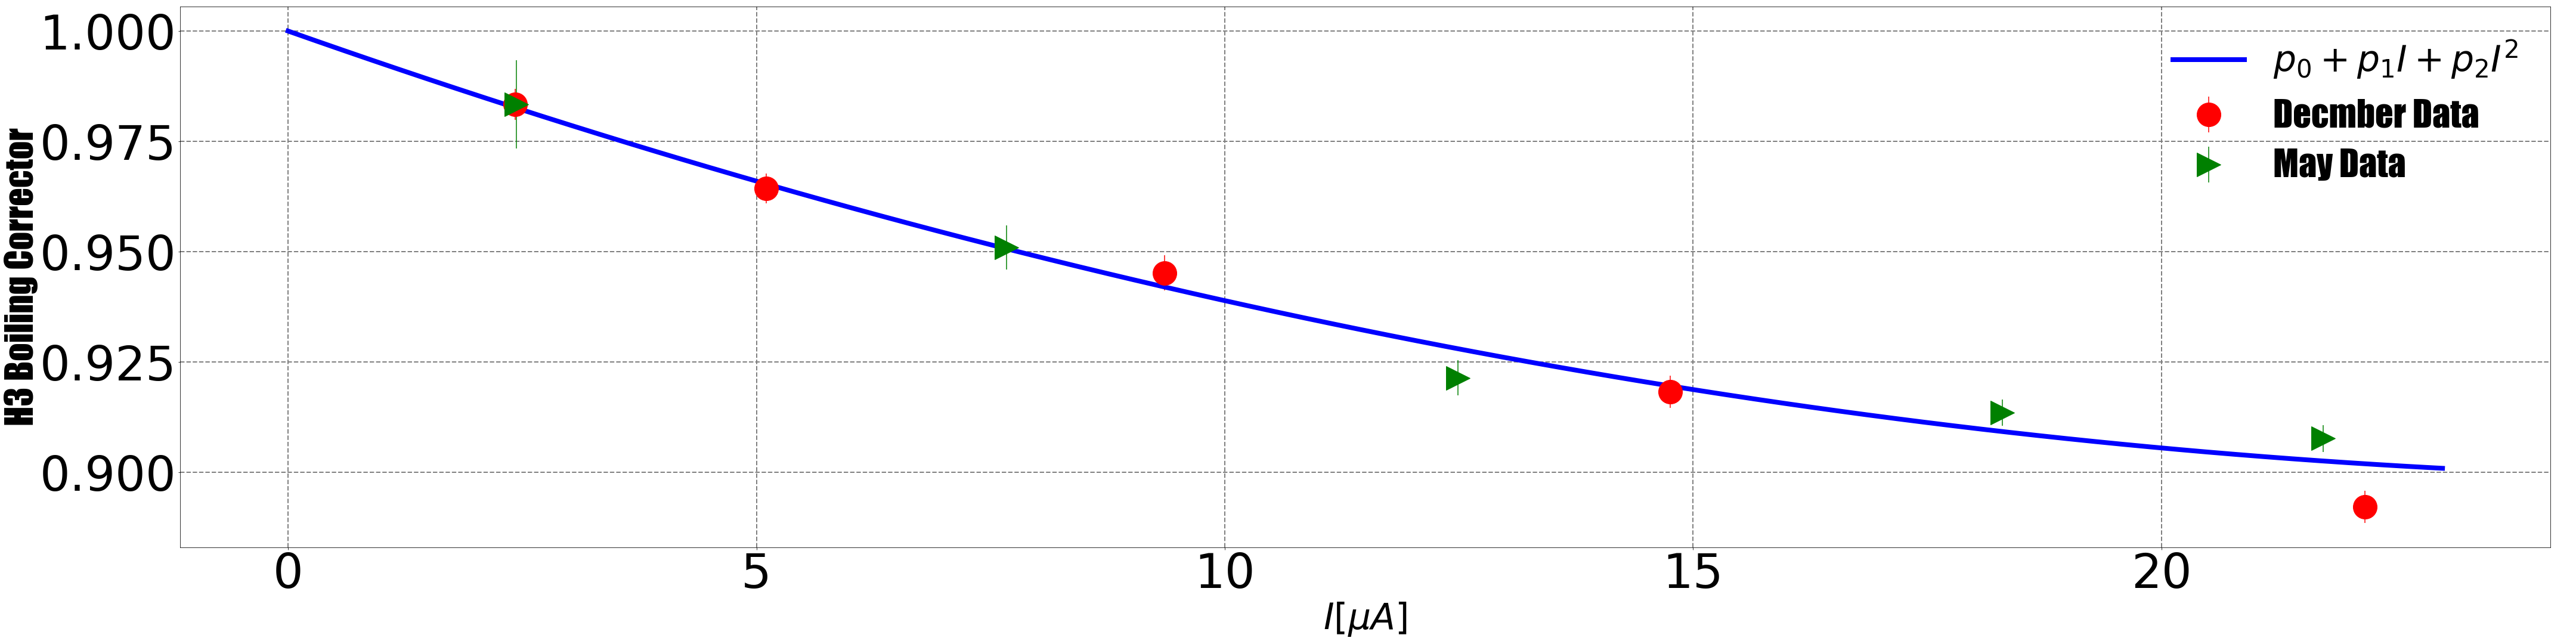
\includegraphics[width=3in]{./boiling_plot/Boiling_H3.png}
\end{minipage}
}\\
\subfigure[Boiling Effect the $^{3}He$]{
\begin{minipage}[t]{1\linewidth}

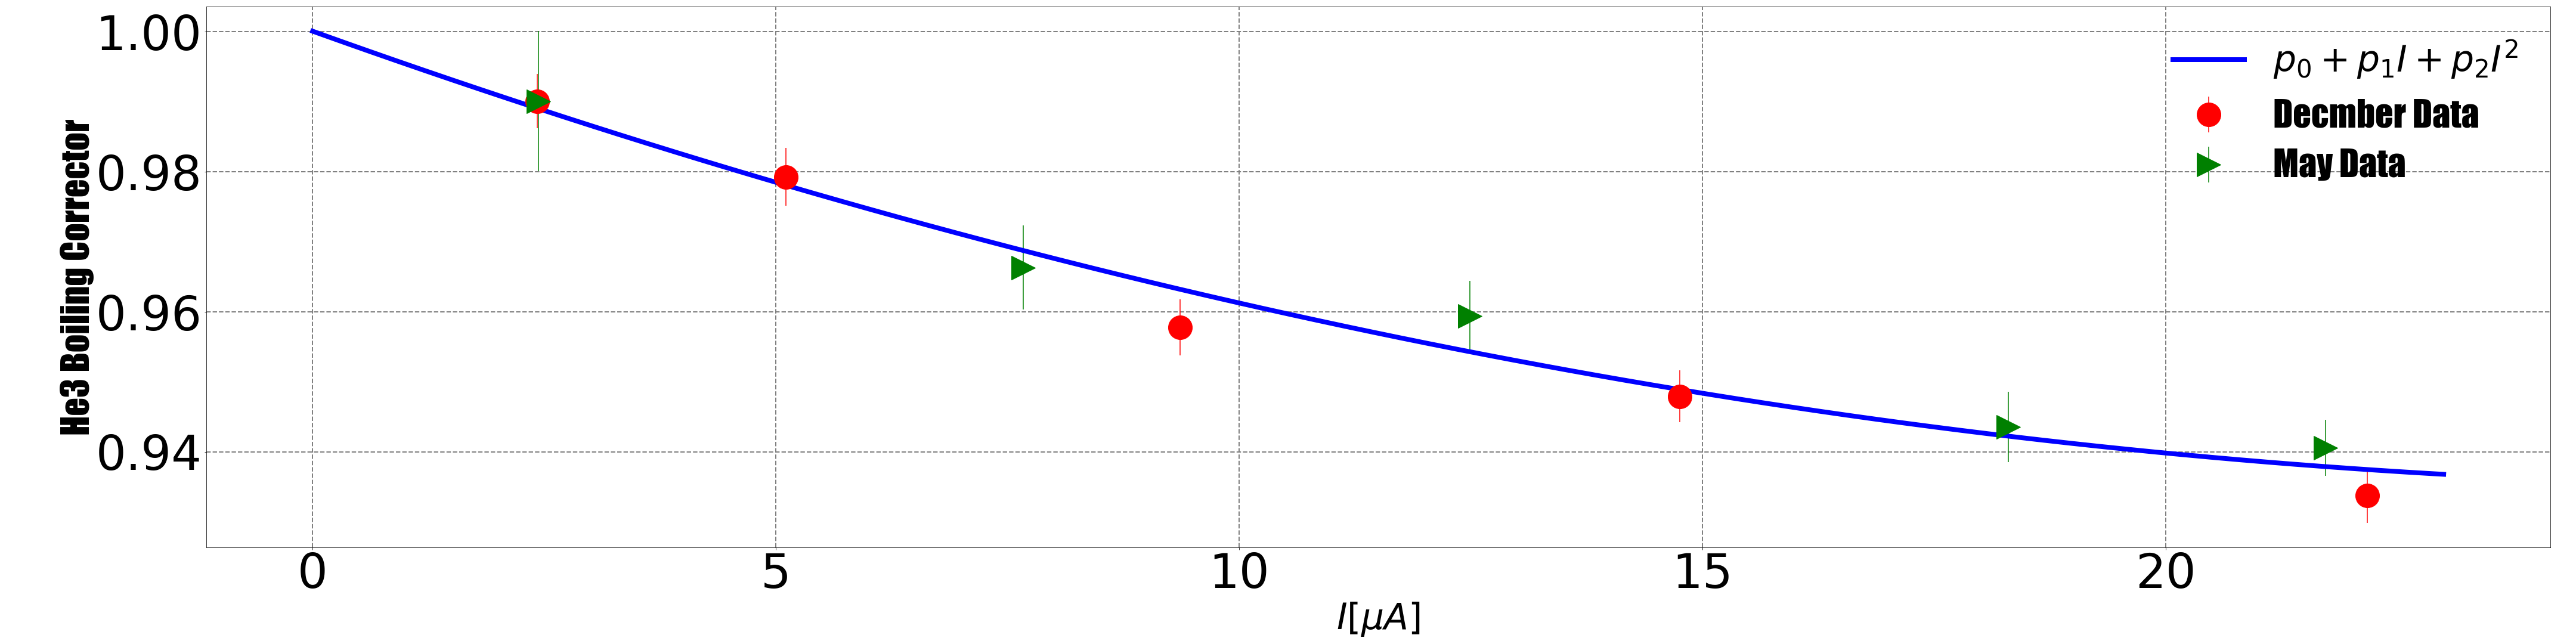
\includegraphics[width=3in]{./boiling_plot/Boiling_He3.png}
\end{minipage}
}

\caption{ the gas target density corrector due to the boiling can be representing equivalently by two ways: Normalized Yield (May Data) or the Normalized Yield ratio(Dec data). The correctors form both methods are shown in the plot and the results agree with each other. For both method, endcap contamination has been taken into consideration and only statistic error is included in the plot  }  \label{boiling_plot1}
\end{figure}
